\documentclass{standalone}
\usepackage{tikz}
\usetikzlibrary{patterns, positioning}
\usepackage[sfdefault]{ClearSans} %% option 'sfdefault' activates Clear Sans as the default text font
\usepackage[T1]{fontenc}

\begin{document}
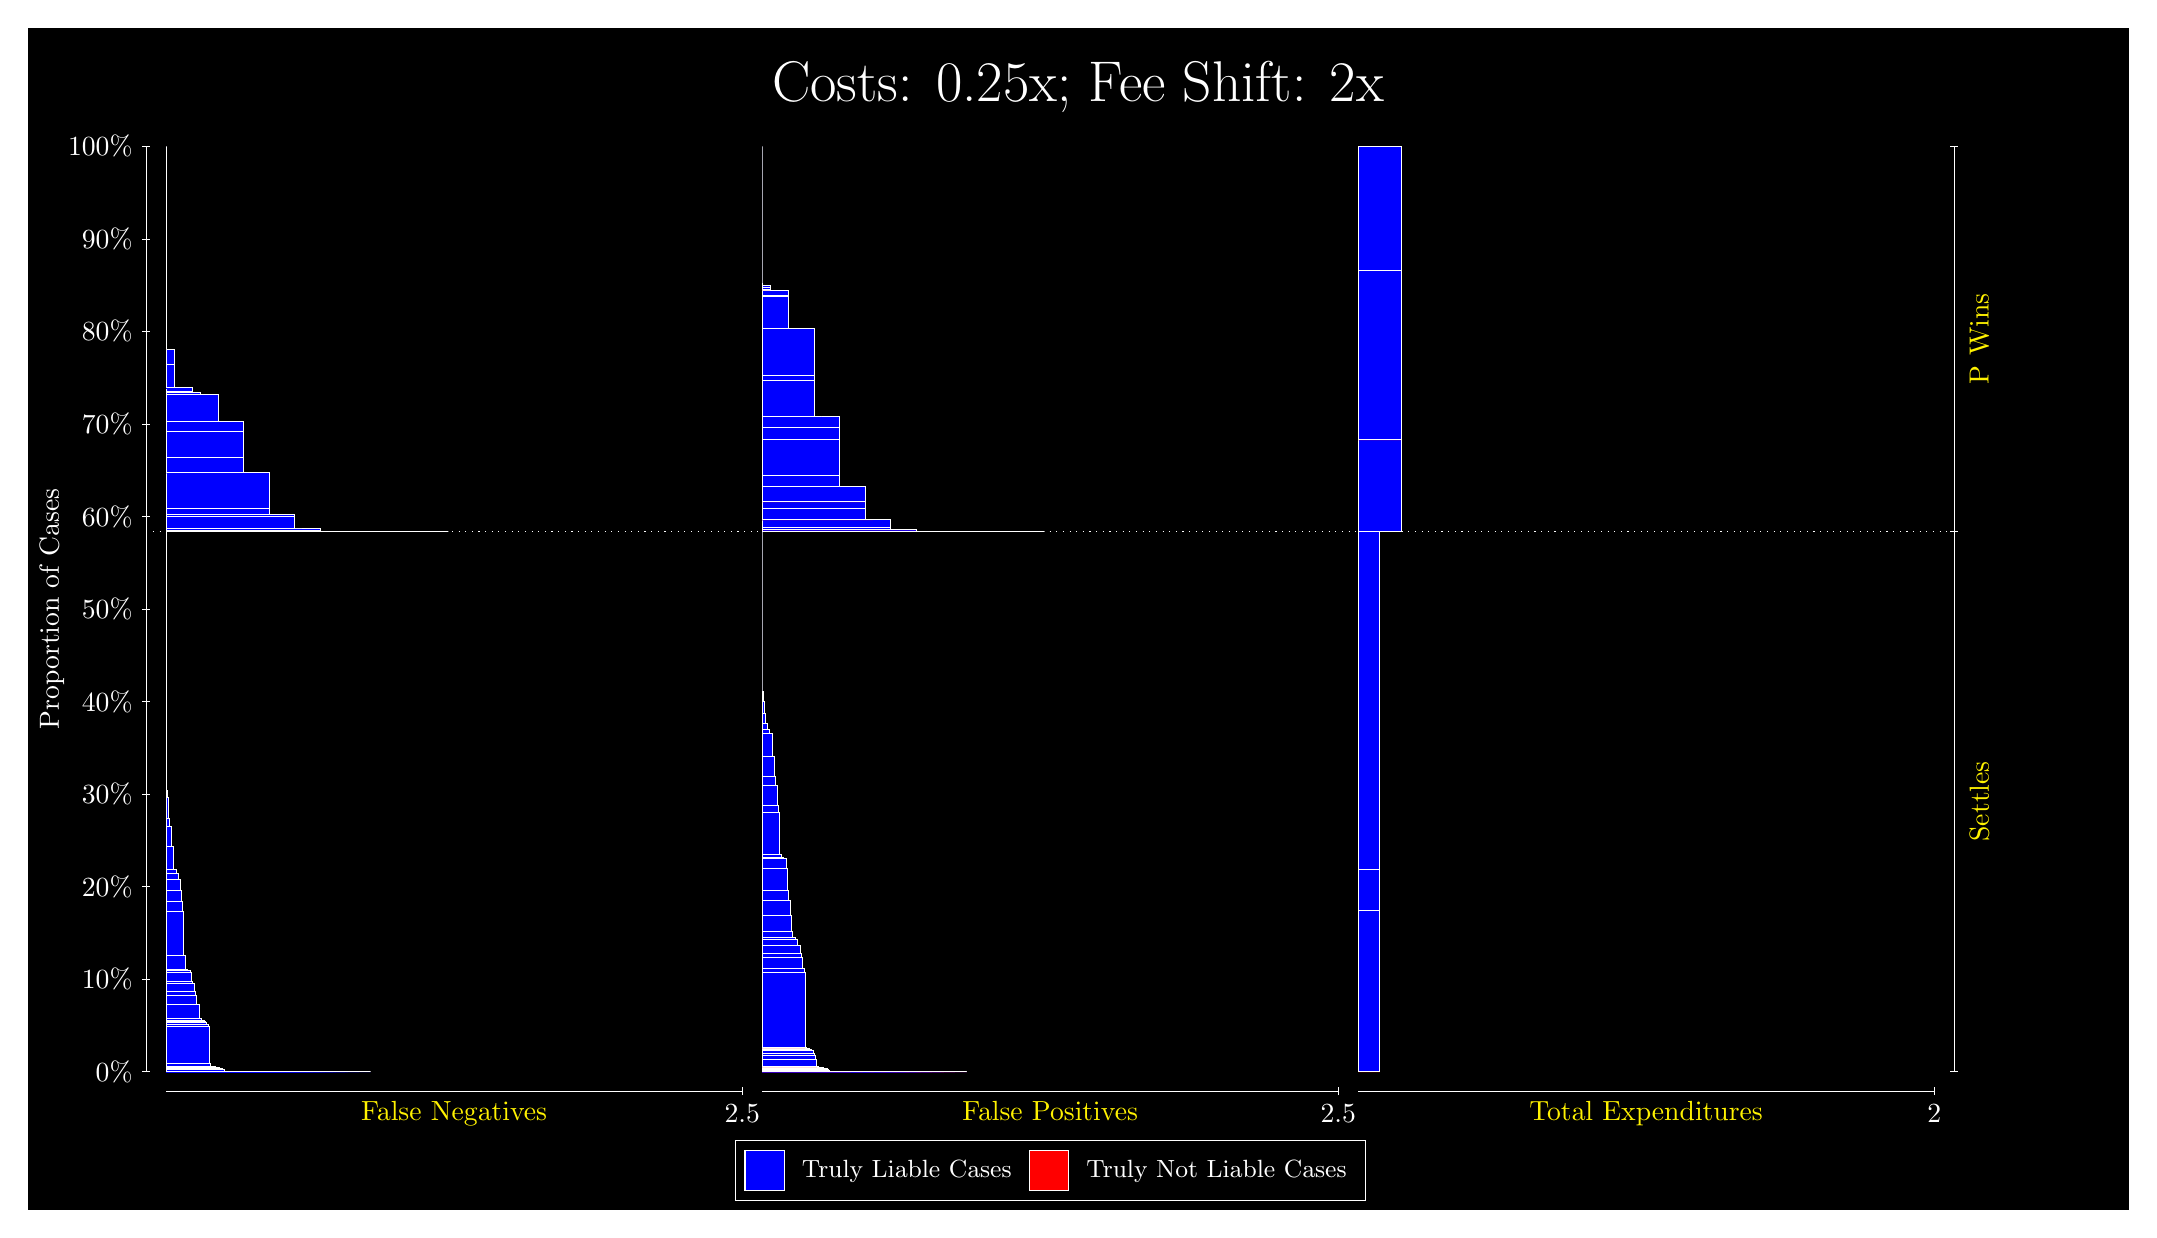
\begin{tikzpicture}
\draw[fill=black] (0,0) rectangle (26.667,15);
\draw[text=white] (0,13.5) rectangle (26.667,15) node[midway] {\huge Costs: 0.25x; Fee Shift: 2x};
\draw[white, very thin] (1.5,1.75) -- (1.5,13.5);
\node[rotate=90, text=white, anchor=center] at (0.3, 7.625) {Proportion of Cases};
\draw[white, very thin] (1.45,1.75) -- (1.55,1.75);
\node[text=white, anchor=east] at (1.45, 1.75) {0\%};
\draw[white, very thin] (1.45,2.925) -- (1.55,2.925);
\node[text=white, anchor=east] at (1.45, 2.925) {10\%};
\draw[white, very thin] (1.45,4.1) -- (1.55,4.1);
\node[text=white, anchor=east] at (1.45, 4.1) {20\%};
\draw[white, very thin] (1.45,5.275) -- (1.55,5.275);
\node[text=white, anchor=east] at (1.45, 5.275) {30\%};
\draw[white, very thin] (1.45,6.45) -- (1.55,6.45);
\node[text=white, anchor=east] at (1.45, 6.45) {40\%};
\draw[white, very thin] (1.45,7.625) -- (1.55,7.625);
\node[text=white, anchor=east] at (1.45, 7.625) {50\%};
\draw[white, very thin] (1.45,8.8) -- (1.55,8.8);
\node[text=white, anchor=east] at (1.45, 8.8) {60\%};
\draw[white, very thin] (1.45,9.975) -- (1.55,9.975);
\node[text=white, anchor=east] at (1.45, 9.975) {70\%};
\draw[white, very thin] (1.45,11.15) -- (1.55,11.15);
\node[text=white, anchor=east] at (1.45, 11.15) {80\%};
\draw[white, very thin] (1.45,12.325) -- (1.55,12.325);
\node[text=white, anchor=east] at (1.45, 12.325) {90\%};
\draw[white, very thin] (1.45,13.5) -- (1.55,13.5);
\node[text=white, anchor=east] at (1.45, 13.5) {100\%};

\draw[white, very thin] (24.457,1.75) -- (24.457,13.5);
\draw[white, very thin] (24.407,1.75) -- (24.507,1.75);
\node[anchor=west] at (24.407, 1.75) {};
\draw[white, very thin] (24.407,8.6123) -- (24.507,8.6123);
\node[anchor=west] at (24.407, 8.6123) {};
\draw[white, very thin] (24.407,13.5) -- (24.507,13.5);
\node[anchor=west] at (24.407, 13.5) {};

\draw[white, very thin, fill=blue] (1.75,1.75) rectangle (4.3482,1.75);
\draw[white, very thin, fill=blue] (1.75,1.75) rectangle (4.2018,1.75);
\draw[white, very thin, fill=blue] (1.75,1.75) rectangle (4.0554,1.75);
\draw[white, very thin, fill=blue] (1.75,1.75) rectangle (4.0229,1.75);
\draw[white, very thin, fill=blue] (1.75,1.75) rectangle (3.9091,1.75);
\draw[white, very thin, fill=blue] (1.75,1.75) rectangle (3.8765,1.75);
\draw[white, very thin, fill=blue] (1.75,1.75) rectangle (3.7627,1.75);
\draw[white, very thin, fill=blue] (1.75,1.75) rectangle (3.7302,1.75);
\draw[white, very thin, fill=blue] (1.75,1.75) rectangle (3.6976,1.75);
\draw[white, very thin, fill=blue] (1.75,1.75) rectangle (3.6163,1.75);
\draw[white, very thin, fill=blue] (1.75,1.75) rectangle (3.5838,1.75);
\draw[white, very thin, fill=blue] (1.75,1.75) rectangle (3.5513,1.75);
\draw[white, very thin, fill=blue] (1.75,1.75) rectangle (3.4699,1.75);
\draw[white, very thin, fill=blue] (1.75,1.75) rectangle (3.4374,1.75);
\draw[white, very thin, fill=blue] (1.75,1.75) rectangle (3.4049,1.75);
\draw[white, very thin, fill=blue] (1.75,1.75) rectangle (3.3723,1.75);
\draw[white, very thin, fill=blue] (1.75,1.75) rectangle (3.3236,1.75);
\draw[white, very thin, fill=blue] (1.75,1.75) rectangle (3.291,1.75);
\draw[white, very thin, fill=blue] (1.75,1.75) rectangle (3.2585,1.75);
\draw[white, very thin, fill=blue] (1.75,1.75) rectangle (3.226,1.75);
\draw[white, very thin, fill=blue] (1.75,1.75) rectangle (3.1772,1.75);
\draw[white, very thin, fill=blue] (1.75,1.75) rectangle (3.1447,1.75);
\draw[white, very thin, fill=blue] (1.75,1.75) rectangle (3.1121,1.75);
\draw[white, very thin, fill=blue] (1.75,1.75) rectangle (3.0796,1.75);
\draw[white, very thin, fill=blue] (1.75,1.75) rectangle (3.0471,1.75);
\draw[white, very thin, fill=blue] (1.75,1.75) rectangle (3.0308,1.75);
\draw[white, very thin, fill=blue] (1.75,1.75) rectangle (2.9983,1.75);
\draw[white, very thin, fill=blue] (1.75,1.75) rectangle (2.9657,1.75);
\draw[white, very thin, fill=blue] (1.75,1.75) rectangle (2.9332,1.75);
\draw[white, very thin, fill=blue] (1.75,1.75) rectangle (2.9007,1.75);
\draw[white, very thin, fill=blue] (1.75,1.75) rectangle (2.8844,1.75);
\draw[white, very thin, fill=blue] (1.75,1.75) rectangle (2.8519,1.75);
\draw[white, very thin, fill=blue] (1.75,1.75) rectangle (2.8194,1.7505);
\draw[white, very thin, fill=blue] (1.75,1.7505) rectangle (2.7868,1.7506);
\draw[white, very thin, fill=blue] (1.75,1.7506) rectangle (2.7543,1.7507);
\draw[white, very thin, fill=blue] (1.75,1.7507) rectangle (2.738,1.7507);
\draw[white, very thin, fill=blue] (1.75,1.7507) rectangle (2.7218,1.7508);
\draw[white, very thin, fill=blue] (1.75,1.7508) rectangle (2.7055,1.7508);
\draw[white, very thin, fill=blue] (1.75,1.7508) rectangle (2.673,1.7509);
\draw[white, very thin, fill=blue] (1.75,1.7509) rectangle (2.6405,1.753);
\draw[white, very thin, fill=blue] (1.75,1.753) rectangle (2.6079,1.7536);
\draw[white, very thin, fill=blue] (1.75,1.7536) rectangle (2.5917,1.7547);
\draw[white, very thin, fill=blue] (1.75,1.7547) rectangle (2.5754,1.7552);
\draw[white, very thin, fill=blue] (1.75,1.7552) rectangle (2.5591,1.7557);
\draw[white, very thin, fill=blue] (1.75,1.7557) rectangle (2.5266,1.7569);
\draw[white, very thin, fill=blue] (1.75,1.7569) rectangle (2.4941,1.7785);
\draw[white, very thin, fill=blue] (1.75,1.7785) rectangle (2.4616,1.7872);
\draw[white, very thin, fill=blue] (1.75,1.7872) rectangle (2.4453,1.7965);
\draw[white, very thin, fill=blue] (1.75,1.7965) rectangle (2.429,1.8026);
\draw[white, very thin, fill=blue] (1.75,1.8026) rectangle (2.4128,1.8043);
\draw[white, very thin, fill=blue] (1.75,1.8043) rectangle (2.3965,1.8095);
\draw[white, very thin, fill=blue] (1.75,1.8095) rectangle (2.3802,1.8125);
\draw[white, very thin, fill=blue] (1.75,1.8125) rectangle (2.3477,1.8143);
\draw[white, very thin, fill=blue] (1.75,1.8143) rectangle (2.3152,1.8588);
\draw[white, very thin, fill=blue] (1.75,1.8588) rectangle (2.2989,2.3297);
\draw[white, very thin, fill=blue] (1.75,2.3297) rectangle (2.2827,2.3515);
\draw[white, very thin, fill=blue] (1.75,2.3515) rectangle (2.2664,2.3748);
\draw[white, very thin, fill=blue] (1.75,2.3748) rectangle (2.2501,2.3937);
\draw[white, very thin, fill=blue] (1.75,2.3937) rectangle (2.2339,2.4067);
\draw[white, very thin, fill=blue] (1.75,2.4067) rectangle (2.2013,2.4269);
\draw[white, very thin, fill=blue] (1.75,2.4269) rectangle (2.1688,2.6054);
\draw[white, very thin, fill=blue] (1.75,2.6054) rectangle (2.1363,2.7186);
\draw[white, very thin, fill=blue] (1.75,2.7186) rectangle (2.12,2.7734);
\draw[white, very thin, fill=blue] (1.75,2.7734) rectangle (2.1037,2.872);
\draw[white, very thin, fill=blue] (1.75,2.872) rectangle (2.0875,2.8988);
\draw[white, very thin, fill=blue] (1.75,2.8988) rectangle (2.0712,3.0075);
\draw[white, very thin, fill=blue] (1.75,3.0075) rectangle (2.055,3.0321);
\draw[white, very thin, fill=blue] (1.75,3.0321) rectangle (2.0224,3.0443);
\draw[white, very thin, fill=blue] (1.75,3.0443) rectangle (1.9899,3.222);
\draw[white, very thin, fill=blue] (1.75,3.222) rectangle (1.9736,3.782);
\draw[white, very thin, fill=blue] (1.75,3.782) rectangle (1.9574,3.9145);
\draw[white, very thin, fill=blue] (1.75,3.9145) rectangle (1.9411,4.0571);
\draw[white, very thin, fill=blue] (1.75,4.0571) rectangle (1.9248,4.1948);
\draw[white, very thin, fill=blue] (1.75,4.1948) rectangle (1.9086,4.2676);
\draw[white, very thin, fill=blue] (1.75,4.2676) rectangle (1.876,4.322);
\draw[white, very thin, fill=blue] (1.75,4.322) rectangle (1.8435,4.606);
\draw[white, very thin, fill=blue] (1.75,4.606) rectangle (1.811,4.8643);
\draw[white, very thin, fill=blue] (1.75,4.8643) rectangle (1.7947,4.9719);
\draw[white, very thin, fill=blue] (1.75,4.9719) rectangle (1.7785,5.2333);
\draw[white, very thin, fill=blue] (1.75,5.2333) rectangle (1.7622,5.3209);
\draw[white, very thin, fill=red] (1.75,5.3209) rectangle (1.75,5.3209);
\draw[white, very thin, fill=blue] (1.75,5.3209) rectangle (1.75,8.6123);
\draw[white, very thin, fill=blue] (1.75,8.6123) rectangle (5.3362,8.6123);
\draw[white, very thin, fill=blue] (1.75,8.6123) rectangle (5.011,8.6123);
\draw[white, very thin, fill=blue] (1.75,8.6123) rectangle (4.6857,8.6123);
\draw[white, very thin, fill=blue] (1.75,8.6123) rectangle (4.3604,8.6127);
\draw[white, very thin, fill=blue] (1.75,8.6127) rectangle (4.0351,8.6156);
\draw[white, very thin, fill=blue] (1.75,8.6156) rectangle (4.0351,8.6172);
\draw[white, very thin, fill=blue] (1.75,8.6172) rectangle (3.8074,8.6172);
\draw[white, very thin, fill=blue] (1.75,8.6172) rectangle (3.7098,8.6282);
\draw[white, very thin, fill=blue] (1.75,8.6282) rectangle (3.7098,8.6528);
\draw[white, very thin, fill=blue] (1.75,8.6528) rectangle (3.4821,8.6528);
\draw[white, very thin, fill=blue] (1.75,8.6528) rectangle (3.4821,8.6528);
\draw[white, very thin, fill=blue] (1.75,8.6528) rectangle (3.3845,8.8046);
\draw[white, very thin, fill=blue] (1.75,8.8046) rectangle (3.3845,8.8283);
\draw[white, very thin, fill=blue] (1.75,8.8283) rectangle (3.1568,8.8283);
\draw[white, very thin, fill=blue] (1.75,8.8283) rectangle (3.1568,8.8283);
\draw[white, very thin, fill=blue] (1.75,8.8283) rectangle (3.1568,8.8283);
\draw[white, very thin, fill=blue] (1.75,8.8283) rectangle (3.0593,8.9002);
\draw[white, very thin, fill=blue] (1.75,8.9002) rectangle (3.0593,9.3549);
\draw[white, very thin, fill=blue] (1.75,9.3549) rectangle (2.8316,9.3549);
\draw[white, very thin, fill=blue] (1.75,9.3549) rectangle (2.8316,9.3549);
\draw[white, very thin, fill=blue] (1.75,9.3549) rectangle (2.734,9.5561);
\draw[white, very thin, fill=blue] (1.75,9.5561) rectangle (2.734,9.884);
\draw[white, very thin, fill=blue] (1.75,9.884) rectangle (2.734,10.009);
\draw[white, very thin, fill=blue] (1.75,10.009) rectangle (2.5063,10.009);
\draw[white, very thin, fill=blue] (1.75,10.009) rectangle (2.5063,10.009);
\draw[white, very thin, fill=blue] (1.75,10.009) rectangle (2.5063,10.01);
\draw[white, very thin, fill=blue] (1.75,10.01) rectangle (2.4087,10.346);
\draw[white, very thin, fill=blue] (1.75,10.346) rectangle (2.181,10.381);
\draw[white, very thin, fill=blue] (1.75,10.381) rectangle (2.181,10.382);
\draw[white, very thin, fill=blue] (1.75,10.382) rectangle (2.0834,10.384);
\draw[white, very thin, fill=blue] (1.75,10.384) rectangle (2.0834,10.434);
\draw[white, very thin, fill=blue] (1.75,10.434) rectangle (2.0834,10.435);
\draw[white, very thin, fill=blue] (1.75,10.435) rectangle (1.8557,10.738);
\draw[white, very thin, fill=blue] (1.75,10.738) rectangle (1.8557,10.921);
\draw[white, very thin, fill=blue] (1.75,10.921) rectangle (1.7581,10.921);
\draw[white, very thin, fill=blue] (1.75,10.921) rectangle (1.7581,10.921);
\draw[white, very thin, fill=red] (1.75,10.921) rectangle (1.75,10.921);
\draw[white, very thin, fill=blue] (1.75,10.921) rectangle (1.75,13.5);
\draw[white, very thin, fill=red] (9.3189,1.75) rectangle (11.917,1.75);
\draw[white, very thin, fill=blue] (9.3189,1.75) rectangle (11.917,1.75);
\draw[white, very thin, fill=red] (9.3189,1.75) rectangle (11.771,1.75);
\draw[white, very thin, fill=blue] (9.3189,1.75) rectangle (11.771,1.75);
\draw[white, very thin, fill=red] (9.3189,1.75) rectangle (11.624,1.75);
\draw[white, very thin, fill=blue] (9.3189,1.75) rectangle (11.624,1.75);
\draw[white, very thin, fill=blue] (9.3189,1.75) rectangle (11.592,1.75);
\draw[white, very thin, fill=red] (9.3189,1.75) rectangle (11.478,1.75);
\draw[white, very thin, fill=blue] (9.3189,1.75) rectangle (11.478,1.75);
\draw[white, very thin, fill=blue] (9.3189,1.75) rectangle (11.445,1.75);
\draw[white, very thin, fill=red] (9.3189,1.75) rectangle (11.332,1.75);
\draw[white, very thin, fill=blue] (9.3189,1.75) rectangle (11.332,1.75);
\draw[white, very thin, fill=blue] (9.3189,1.75) rectangle (11.299,1.75);
\draw[white, very thin, fill=blue] (9.3189,1.75) rectangle (11.266,1.75);
\draw[white, very thin, fill=red] (9.3189,1.75) rectangle (11.185,1.75);
\draw[white, very thin, fill=blue] (9.3189,1.75) rectangle (11.185,1.75);
\draw[white, very thin, fill=blue] (9.3189,1.75) rectangle (11.153,1.75);
\draw[white, very thin, fill=blue] (9.3189,1.75) rectangle (11.12,1.75);
\draw[white, very thin, fill=red] (9.3189,1.75) rectangle (11.039,1.75);
\draw[white, very thin, fill=blue] (9.3189,1.75) rectangle (11.039,1.75);
\draw[white, very thin, fill=blue] (9.3189,1.75) rectangle (11.006,1.75);
\draw[white, very thin, fill=blue] (9.3189,1.75) rectangle (10.974,1.75);
\draw[white, very thin, fill=blue] (9.3189,1.75) rectangle (10.941,1.75);
\draw[white, very thin, fill=red] (9.3189,1.75) rectangle (10.892,1.75);
\draw[white, very thin, fill=blue] (9.3189,1.75) rectangle (10.892,1.75);
\draw[white, very thin, fill=blue] (9.3189,1.75) rectangle (10.86,1.75);
\draw[white, very thin, fill=blue] (9.3189,1.75) rectangle (10.827,1.75);
\draw[white, very thin, fill=blue] (9.3189,1.75) rectangle (10.795,1.75);
\draw[white, very thin, fill=red] (9.3189,1.75) rectangle (10.746,1.75);
\draw[white, very thin, fill=blue] (9.3189,1.75) rectangle (10.746,1.75);
\draw[white, very thin, fill=blue] (9.3189,1.75) rectangle (10.714,1.75);
\draw[white, very thin, fill=blue] (9.3189,1.75) rectangle (10.681,1.75);
\draw[white, very thin, fill=blue] (9.3189,1.75) rectangle (10.648,1.75);
\draw[white, very thin, fill=blue] (9.3189,1.75) rectangle (10.616,1.75);
\draw[white, very thin, fill=red] (9.3189,1.75) rectangle (10.6,1.75);
\draw[white, very thin, fill=blue] (9.3189,1.75) rectangle (10.6,1.75);
\draw[white, very thin, fill=blue] (9.3189,1.75) rectangle (10.567,1.75);
\draw[white, very thin, fill=blue] (9.3189,1.75) rectangle (10.535,1.7501);
\draw[white, very thin, fill=blue] (9.3189,1.7501) rectangle (10.502,1.7502);
\draw[white, very thin, fill=blue] (9.3189,1.7502) rectangle (10.47,1.7503);
\draw[white, very thin, fill=red] (9.3189,1.7503) rectangle (10.453,1.7503);
\draw[white, very thin, fill=blue] (9.3189,1.7503) rectangle (10.453,1.7504);
\draw[white, very thin, fill=blue] (9.3189,1.7504) rectangle (10.421,1.7505);
\draw[white, very thin, fill=blue] (9.3189,1.7505) rectangle (10.388,1.7505);
\draw[white, very thin, fill=blue] (9.3189,1.7505) rectangle (10.356,1.7508);
\draw[white, very thin, fill=blue] (9.3189,1.7508) rectangle (10.323,1.7536);
\draw[white, very thin, fill=red] (9.3189,1.7536) rectangle (10.307,1.7536);
\draw[white, very thin, fill=blue] (9.3189,1.7536) rectangle (10.307,1.7548);
\draw[white, very thin, fill=blue] (9.3189,1.7548) rectangle (10.291,1.7561);
\draw[white, very thin, fill=blue] (9.3189,1.7561) rectangle (10.274,1.7566);
\draw[white, very thin, fill=blue] (9.3189,1.7566) rectangle (10.242,1.7567);
\draw[white, very thin, fill=blue] (9.3189,1.7567) rectangle (10.209,1.7574);
\draw[white, very thin, fill=blue] (9.3189,1.7574) rectangle (10.177,1.7642);
\draw[white, very thin, fill=red] (9.3189,1.7642) rectangle (10.161,1.7642);
\draw[white, very thin, fill=blue] (9.3189,1.7642) rectangle (10.161,1.7824);
\draw[white, very thin, fill=blue] (9.3189,1.7824) rectangle (10.144,1.7876);
\draw[white, very thin, fill=blue] (9.3189,1.7876) rectangle (10.128,1.7946);
\draw[white, very thin, fill=blue] (9.3189,1.7946) rectangle (10.095,1.7995);
\draw[white, very thin, fill=blue] (9.3189,1.7995) rectangle (10.063,1.8016);
\draw[white, very thin, fill=blue] (9.3189,1.8016) rectangle (10.03,1.8125);
\draw[white, very thin, fill=red] (9.3189,1.8125) rectangle (10.014,1.8125);
\draw[white, very thin, fill=blue] (9.3189,1.8125) rectangle (10.014,1.9055);
\draw[white, very thin, fill=blue] (9.3189,1.9055) rectangle (9.9979,1.9554);
\draw[white, very thin, fill=blue] (9.3189,1.9554) rectangle (9.9816,1.9804);
\draw[white, very thin, fill=blue] (9.3189,1.9804) rectangle (9.9654,2.0185);
\draw[white, very thin, fill=blue] (9.3189,2.0185) rectangle (9.9491,2.0377);
\draw[white, very thin, fill=blue] (9.3189,2.0377) rectangle (9.9166,2.0401);
\draw[white, very thin, fill=blue] (9.3189,2.0401) rectangle (9.884,2.0522);
\draw[white, very thin, fill=red] (9.3189,2.0522) rectangle (9.8678,2.0522);
\draw[white, very thin, fill=blue] (9.3189,2.0522) rectangle (9.8678,3.0111);
\draw[white, very thin, fill=blue] (9.3189,3.0111) rectangle (9.8515,3.067);
\draw[white, very thin, fill=blue] (9.3189,3.067) rectangle (9.8353,3.1969);
\draw[white, very thin, fill=blue] (9.3189,3.1969) rectangle (9.819,3.2475);
\draw[white, very thin, fill=blue] (9.3189,3.2475) rectangle (9.8027,3.3474);
\draw[white, very thin, fill=blue] (9.3189,3.3474) rectangle (9.7702,3.4346);
\draw[white, very thin, fill=blue] (9.3189,3.4346) rectangle (9.7377,3.4598);
\draw[white, very thin, fill=blue] (9.3189,3.4598) rectangle (9.7051,3.5296);
\draw[white, very thin, fill=blue] (9.3189,3.5296) rectangle (9.6889,3.7334);
\draw[white, very thin, fill=blue] (9.3189,3.7334) rectangle (9.6726,3.9197);
\draw[white, very thin, fill=blue] (9.3189,3.9197) rectangle (9.6563,4.0538);
\draw[white, very thin, fill=blue] (9.3189,4.0538) rectangle (9.6401,4.326);
\draw[white, very thin, fill=blue] (9.3189,4.326) rectangle (9.6238,4.4624);
\draw[white, very thin, fill=blue] (9.3189,4.4624) rectangle (9.5913,4.4755);
\draw[white, very thin, fill=blue] (9.3189,4.4755) rectangle (9.5588,4.515);
\draw[white, very thin, fill=blue] (9.3189,4.515) rectangle (9.5425,5.0414);
\draw[white, very thin, fill=blue] (9.3189,5.0414) rectangle (9.5262,5.129);
\draw[white, very thin, fill=blue] (9.3189,5.129) rectangle (9.51,5.3904);
\draw[white, very thin, fill=blue] (9.3189,5.3904) rectangle (9.4937,5.498);
\draw[white, very thin, fill=blue] (9.3189,5.498) rectangle (9.4774,5.7563);
\draw[white, very thin, fill=blue] (9.3189,5.7563) rectangle (9.4449,6.0403);
\draw[white, very thin, fill=blue] (9.3189,6.0403) rectangle (9.4124,6.0947);
\draw[white, very thin, fill=blue] (9.3189,6.0947) rectangle (9.3799,6.1675);
\draw[white, very thin, fill=blue] (9.3189,6.1675) rectangle (9.3636,6.3052);
\draw[white, very thin, fill=blue] (9.3189,6.3052) rectangle (9.3473,6.4478);
\draw[white, very thin, fill=blue] (9.3189,6.4478) rectangle (9.3311,6.5803);
\draw[white, very thin, fill=blue] (9.3189,6.5803) rectangle (9.3189,8.6123);
\draw[white, very thin, fill=red] (9.3189,8.6123) rectangle (12.905,8.6123);
\draw[white, very thin, fill=blue] (9.3189,8.6123) rectangle (12.905,8.6123);
\draw[white, very thin, fill=red] (9.3189,8.6123) rectangle (12.58,8.6123);
\draw[white, very thin, fill=blue] (9.3189,8.6123) rectangle (12.58,8.6123);
\draw[white, very thin, fill=red] (9.3189,8.6123) rectangle (12.255,8.6123);
\draw[white, very thin, fill=blue] (9.3189,8.6123) rectangle (12.255,8.6123);
\draw[white, very thin, fill=blue] (9.3189,8.6123) rectangle (11.929,8.6124);
\draw[white, very thin, fill=blue] (9.3189,8.6124) rectangle (11.929,8.6124);
\draw[white, very thin, fill=red] (9.3189,8.6124) rectangle (11.929,8.6124);
\draw[white, very thin, fill=blue] (9.3189,8.6124) rectangle (11.929,8.6125);
\draw[white, very thin, fill=blue] (9.3189,8.6125) rectangle (11.604,8.6136);
\draw[white, very thin, fill=red] (9.3189,8.6136) rectangle (11.604,8.6136);
\draw[white, very thin, fill=blue] (9.3189,8.6136) rectangle (11.604,8.6143);
\draw[white, very thin, fill=blue] (9.3189,8.6143) rectangle (11.604,8.6148);
\draw[white, very thin, fill=red] (9.3189,8.6148) rectangle (11.376,8.6148);
\draw[white, very thin, fill=blue] (9.3189,8.6148) rectangle (11.376,8.6148);
\draw[white, very thin, fill=blue] (9.3189,8.6148) rectangle (11.279,8.6311);
\draw[white, very thin, fill=red] (9.3189,8.6311) rectangle (11.279,8.6311);
\draw[white, very thin, fill=blue] (9.3189,8.6311) rectangle (11.279,8.6361);
\draw[white, very thin, fill=blue] (9.3189,8.6361) rectangle (11.051,8.6361);
\draw[white, very thin, fill=red] (9.3189,8.6361) rectangle (11.051,8.6361);
\draw[white, very thin, fill=blue] (9.3189,8.6361) rectangle (11.051,8.6361);
\draw[white, very thin, fill=blue] (9.3189,8.6361) rectangle (10.953,8.6618);
\draw[white, very thin, fill=red] (9.3189,8.6618) rectangle (10.953,8.6618);
\draw[white, very thin, fill=blue] (9.3189,8.6618) rectangle (10.953,8.7576);
\draw[white, very thin, fill=blue] (9.3189,8.7576) rectangle (10.726,8.7576);
\draw[white, very thin, fill=red] (9.3189,8.7576) rectangle (10.726,8.7576);
\draw[white, very thin, fill=blue] (9.3189,8.7576) rectangle (10.726,8.7576);
\draw[white, very thin, fill=blue] (9.3189,8.7576) rectangle (10.628,8.9033);
\draw[white, very thin, fill=blue] (9.3189,8.9033) rectangle (10.628,8.9888);
\draw[white, very thin, fill=red] (9.3189,8.9888) rectangle (10.628,8.9888);
\draw[white, very thin, fill=blue] (9.3189,8.9888) rectangle (10.628,9.1826);
\draw[white, very thin, fill=blue] (9.3189,9.1826) rectangle (10.4,9.1826);
\draw[white, very thin, fill=blue] (9.3189,9.1826) rectangle (10.4,9.1826);
\draw[white, very thin, fill=red] (9.3189,9.1826) rectangle (10.4,9.1826);
\draw[white, very thin, fill=blue] (9.3189,9.1826) rectangle (10.4,9.1826);
\draw[white, very thin, fill=blue] (9.3189,9.1826) rectangle (10.303,9.3166);
\draw[white, very thin, fill=blue] (9.3189,9.3166) rectangle (10.303,9.7845);
\draw[white, very thin, fill=blue] (9.3189,9.7845) rectangle (10.303,9.9366);
\draw[white, very thin, fill=blue] (9.3189,9.9366) rectangle (10.303,10.072);
\draw[white, very thin, fill=blue] (9.3189,10.072) rectangle (10.075,10.072);
\draw[white, very thin, fill=blue] (9.3189,10.072) rectangle (10.075,10.072);
\draw[white, very thin, fill=red] (9.3189,10.072) rectangle (10.075,10.072);
\draw[white, very thin, fill=blue] (9.3189,10.072) rectangle (10.075,10.072);
\draw[white, very thin, fill=blue] (9.3189,10.072) rectangle (9.9776,10.526);
\draw[white, very thin, fill=blue] (9.3189,10.526) rectangle (9.9776,10.597);
\draw[white, very thin, fill=blue] (9.3189,10.597) rectangle (9.9776,11.191);
\draw[white, very thin, fill=blue] (9.3189,11.191) rectangle (9.7499,11.191);
\draw[white, very thin, fill=red] (9.3189,11.191) rectangle (9.7499,11.191);
\draw[white, very thin, fill=blue] (9.3189,11.191) rectangle (9.7499,11.192);
\draw[white, very thin, fill=blue] (9.3189,11.192) rectangle (9.6523,11.591);
\draw[white, very thin, fill=blue] (9.3189,11.591) rectangle (9.6523,11.606);
\draw[white, very thin, fill=blue] (9.3189,11.606) rectangle (9.6523,11.678);
\draw[white, very thin, fill=blue] (9.3189,11.678) rectangle (9.4246,11.678);
\draw[white, very thin, fill=blue] (9.3189,11.678) rectangle (9.4246,11.679);
\draw[white, very thin, fill=red] (9.3189,11.679) rectangle (9.4246,11.679);
\draw[white, very thin, fill=blue] (9.3189,11.679) rectangle (9.4246,11.713);
\draw[white, very thin, fill=blue] (9.3189,11.713) rectangle (9.4246,11.73);
\draw[white, very thin, fill=blue] (9.3189,11.73) rectangle (9.327,11.766);
\draw[white, very thin, fill=red] (9.3189,11.766) rectangle (9.3189,11.766);
\draw[white, very thin, fill=blue] (9.3189,11.766) rectangle (9.3189,13.5);
\draw[white, very thin, fill=red] (16.888,1.75) rectangle (17.162,1.75);
\draw[white, very thin, fill=blue] (16.888,1.75) rectangle (17.162,3.8032);
\draw[white, very thin, fill=red] (16.888,3.8032) rectangle (17.162,3.8032);
\draw[white, very thin, fill=blue] (16.888,3.8032) rectangle (17.162,4.3176);
\draw[white, very thin, fill=red] (16.888,4.3176) rectangle (17.162,4.3176);
\draw[white, very thin, fill=blue] (16.888,4.3176) rectangle (17.162,8.6123);
\draw[white, very thin, fill=red] (16.888,8.6123) rectangle (17.437,8.6123);
\draw[white, very thin, fill=blue] (16.888,8.6123) rectangle (17.437,9.7732);
\draw[white, very thin, fill=red] (16.888,9.7732) rectangle (17.437,9.7732);
\draw[white, very thin, fill=blue] (16.888,9.7732) rectangle (17.437,11.931);
\draw[white, very thin, fill=red] (16.888,11.931) rectangle (17.437,11.931);
\draw[white, very thin, fill=blue] (16.888,11.931) rectangle (17.437,13.5);
\draw[white, dotted] (1.5,8.6123) -- (24.457,8.6123);
\draw[white, very thin] (1.75,1.5) -- (9.0689,1.5);
\node[text=yellow, anchor=north] at (5.4094, 1.5) {False Negatives};
\draw[white, very thin] (9.0689,1.45) -- (9.0689,1.55);
\node[text=white, anchor=north] at (9.0689, 1.45) {2.5};

\draw[white, very thin] (9.3189,1.5) -- (16.638,1.5);
\node[text=yellow, anchor=north] at (12.978, 1.5) {False Positives};
\draw[white, very thin] (16.638,1.45) -- (16.638,1.55);
\node[text=white, anchor=north] at (16.638, 1.45) {2.5};

\draw[white, very thin] (16.888,1.5) -- (24.207,1.5);
\node[text=yellow, anchor=north] at (20.547, 1.5) {Total Expenditures};
\draw[white, very thin] (24.207,1.45) -- (24.207,1.55);
\node[text=white, anchor=north] at (24.207, 1.45) {2};

\node[text=yellow, centered, rotate=90] at (24.777, 5.1811) {Settles};
\node[text=yellow, centered, rotate=90] at (24.777, 11.056) {P Wins};

\draw (12.978300999999998,1.5) node[draw=none] (baseCoordinate) {};
\begin{scope}[align=center]
        \matrix[scale=0.5, draw=white, below=0.5cm of baseCoordinate, nodes={draw}, column sep=0.1cm]{
            \node[rectangle, draw, minimum width=0.5cm, minimum height=0.5cm, fill=blue] {}; &
            \node[draw=none, font=\small, text=white] (B) {Truly Liable Cases}; &
            \node[rectangle, draw, minimum width=0.5cm, minimum height=0.5cm, fill=red] {}; &
            \node[draw=none, font=\small, text=white] (B) {Truly Not Liable Cases}; \\
            };
\end{scope}

\end{tikzpicture}
\end{document}